The master controller represents a collection of controllers, which all have the role of handling input from the user and translate it into
the correct action. These controllers typically interact with the \texttt{GestureHand} class to check if a certain hand state-criterion
is met, utilize its utility functions and check for changes every frame. The \texttt{GestureHand} will be covered more in depth in section~\vref{sec:gesturehand_class}, 
but can in short be described as a class which is instantiated once per hand and keeps track of what potential gesture the hands are performing, the origin coordinates
for the potential gestures and other useful hand-specific information. 

Another important component in the controllers, with the \texttt{AnnotationFormController} as an exception, is how they all relies on the Update-function, 
which is called in a set order by the Unity runtime environment on every frame. During the update call these controllers checks for input relevant for its 
purposes. The following four sections will cover the controllers that the master controller contains.

\subsection{The Rotation Controller}
The \texttt{RotationController} is a script component of the \texttt{MasterController} and its primary function to handle user input related to rotation.
\texttt{RotationController} contains a number of instance variables, which will be described below. Some of these variables have a public access modifier, as
this allows their values to be seen and edited from the Unity Inspector view (see figure~\vref{fig:unity_inspector} for an example). Variables that does not
have this requirement, and is which should not be accessed from other parts of the application, are given a private access modifier.

\begin{itemize}
    \item \texttt{public GestureHand leftHand, rightHand} - Stores the \texttt{GestureHand} instances that represents the left and right hand.
    \item \texttt{public float sensitivity} - A float-point multiplier that determines the sensitivity of the rotational actions. 
                                              All statements that rotates the camera is multiplied by this variable's value, which by default is 100.0.
    \item \texttt{public float clampAngle} - An absolute value in degrees for the maximum rotation allowed along in y-axis. 
                                            Its default is 90.0 (degrees), meaning that the user can rotate from looking straight ahead (0.0 degrees on the y-axis) to 
                                            straight up (90.0 degrees on the y-axis) and straight down (-90.0 degrees on the y-axis). Note that this rotational 
                                            limitation along the y-axis is in place to prevent the user from rotating the cameras (and the enire \texttt{MasterController}) 
                                            "upside-down". %Include an illustration?                                         
    \item \texttt{private float rotX, rotY} - The floatpoint variables rotX and rotY are intermediate values that stores the rotation of the \texttt{MasterController} (and thus the
                                              cameras) and is used to calculate the new rotation quaternion that is applied to the \texttt{MasterController}'s transform 
                                              every frame. Note that \texttt{RotationController} only allows rotation
                                              along the x-axis (left-and-right) and y-axis (up-and-down), and not along the z-axis (a "barrel roll" rotation). 
    \item \texttt{private InteractionBox iBox} - The \texttt{InteractionBox} class is a Leap Motion abstraction for the area (i.e the "box") above/in front of 
                                                the Leap Motion device that is interactable (i.e where the device can detect and track the hands), 
                                                and is used for normalizing purposes. 
                                                This variable holds a reference to the latest InteractionBox-object, which is updated on every Leap Motion-frame by
                                                retrieving it from the Leap Motion \texttt{Frame} object (see table~\vref{table:annotation_visibility_code} for an example).  
\end{itemize}

During its update function \texttt{RotationController} both checks for mouse movements and whether the pinch gesture is performed by either hand.

Mouse movements are retrieved by calling the unity-function \texttt{Input.GetAxis(string axisName)} once per axis (i.e twice to get the x- and y axis). 
The return value of this function is in the range -1 and 1 for each axis, which signifies in what direction the mouse is moving and at what speed. 
If \texttt{Input.GetAxis("Mouse X")} e.g.~returns "-0.01" the mouse is moving very slowly to the left, while "1.0" would mean that is moves as fast as possible to the right. 
If calling GetAxis with the x-axis and the y-axis both yield 0, then the mouse is not moving and no rotation is performed.

\begin{table}
\label{table:rotation_mouse_code}
\lstset{style=csharp}
\begin{lstlisting}
public float sensitivity = 100.0f;
private float rotX, rotY = 0.0f;

void Update() { // Update is called every frame
    trackMouse();
    [...]
    
    // Create new rotation quaternion and replace the rotation of the 
    // MasterController's transform. 
    Quaternion localRotation = Quaternion.Euler(rotX, rotY, 0.0f);
    transform.rotation = localRotation;         
}

private void trackMouse() {
    float mouseX = Input.GetAxis("Mouse X");  // Get x-axis mouse movement
    float mouseY = -Input.GetAxis("Mouse Y");// Get y-axis mouse movement

    rotY += mouseX * sensitivity * Time.deltaTime; // Transform mouse movements
    rotX += mouseY * sensitivity * Time.deltaTime; // to rotations  
}                                                                                
\end{lstlisting}
\caption[How mouse movement is captured and transformed to rotations]{How mouse movement is captured and transformed to rotations.} 
\end{table}

% // Create new position quaternion and update the MasterController's position
%     Quaternion newRot = Quaternion.Euler(rotX, rotY, 0.0f);                          
%     transform.rotation = newRot;  

Before applying the captured mouse movements to the rotation it is multiplied by the sensitivity variable outlined above, and by \texttt{Time.deltaTime}.
\texttt{Time.deltaTime} is another function in the Unity framework and returns the time in seconds it took to complete the last frame.
By applying this to the equation we make the calculation frame rate independent and essentially expresses that we want to rotate X amount per second, instead of
X amount per frame.

The pinch gesture, which is used for rotation, is captured in a similar fashion. The update function checks for the pinch state, and if its detected
it tracks the hand position within the interaction box (i.e the area above/in front of the Leap Motion device). 
Just as the variables \texttt{mouseX} and \texttt{mouseY} is captured in table~\vref{table:rotation_mouse_code} the variables 
\texttt{handX} and \texttt{handY} are captured, but somewhat differently. These two variables are calculated by obtaining the hand's palm position within the interaction box
and subtracting the origin point, i.e the point were the current pinch gesture started (see table~\vref{table:rotation_gesture_code}). 
After this is done they are, like with the mouse movement, multiplied by the \texttt{sensitivity} variable and \texttt{Time.deltaTime}. 


\begin{table}
\label{table:rotation_gesture_code}
\lstset{style=csharp}
\begin{lstlisting}
public GestureHand leftHand, righthand; 
public float sensitivity = 100.0f;
private float rotX, rotY = 0.0f;

void Update() {
    trackMouse();

    bool leftPinch = false, rightPinch = false;
    
    if (leftHand.getGestureType() == GestureHand.HandState.PINCH)
        leftPinch = true;
    if (rightHand.getGestureType() == GestureHand.HandState.PINCH)
        rightPinch = true;

    if (leftPinch || rightPinch) {
        Frame frame = LeapBehavior.getLastFrame();
        iBox = frame.InteractionBox;
        for (int i = 0; i < frame.Hands.Count; i++) {
            Hand hand = frame.Hands[i];

            if (hand.IsLeft && leftPinch)
                TrackPinch(hand, leftHand.GetGestureOriginPosition());

            if (!hand.IsLeft && rightPinch)
                TrackPinch(hand, rightHand.GetGestureOriginPosition());
        }
    }
    
    // Create new rotation quaternion and replace the rotation of the 
    // MasterController's transform. 
    Quaternion localRotation = Quaternion.Euler(rotX, rotY, 0.0f);
    transform.rotation = localRotation;         
}

private void TrackPinch(Hand hand, Leap.Vector originCoordinates)
{       
    // Get position, convert from right to left hand coordinates, normalize
    Leap.Vector leapPoint = hand.StabilizedPalmPosition * -1.0f;
    Leap.Vector normalizedPoint = iBox.NormalizePoint(leapPoint, false);

    float handX = normalizedPoint.x - originCoordinates.x; // Find x-offset
    float handY = normalizedPoint.y - originCoordinates.y; // Find y-offset

    // Transform hand movement to rotation
    rotX += -handY * sensitivity * Time.deltaTime;
    rotY +=  handX * sensitivity * Time.deltaTime;
}                                                                                  
\end{lstlisting}
\caption[How the pinch gesture is captured and transformed to rotations]{How the pinch gesture is captured and transformed to rotations. 
            Note that the implementation code looks somewhat different (e.g.~Some shorter variable names in this table.)} 
\end{table}

% Illustration idea: Detector -> *detects gesture* -> GestureHand's activate <- Controllers check hand state. 

\subsection{The Movement Controller}
The \texttt{MovementController} is another script component of the \texttt{MasterController}, and relates to the movement of the user. 
This controller has many similarities with the \texttt{RotationController}, covered in the previous section, as it has very similar
code for hand detection in the update method. If one of the hands have a different state than NONE, the \texttt{TrackHandMovement} 
(see table~\vref{table:movement_gesture_code}) is called. In this function the hand position is obtained and a number of conditions are checked for:

\begin{enumerate}
    \item Is the combined gesture scheme used AND is the palm-down gesture active?
    \item Is the combined gesture scheme NOT used AND is the palm-down gesture active?
    \item Is the combined gesture scheme NOT used AND is the palm-side gesture active?
    \item Is the combined gesture scheme NOT used AND is the fist gesture active?
\end{enumerate}

If any of these criteria are met the appropriate action is taken. 
For the last criterion this would mean going forward by X, where X is positive or negative float point number, 
and is the result of (current coordinates - origin coordinates). Also not that although only one of these cases can trigger for one hand, the user can 
perform different (or the same) gesture with each hand, and thus perform more of these cases at the same time.

\begin{table}
\label{table:movement_gesture_code}
\lstset{style=csharp}
\begin{lstlisting}
private void TrackHandMovement(Hand hand, GestureHand gestureHand)
{
    // Get position, convert from right to left hand coordinates, normalize
    Leap.Vector leapPoint = hand.StabilizedPalmPosition * -1.0f;
    Leap.Vector normalizedPoint = iBox.NormalizePoint(leapPoint, false);

    // True if movement along the x-, y- and z-axis are handle by one gesture instead of three, false otherwise.
    if (gestureHand.getCombineGestures()) 
    {
        if (gestureHand.getGestureType() == HandState.PALM_DOWN)
        {
            transform.position += transform.up * speed * (normalizedPoint.y - gestureHand.GetGestureOriginPosition().y) * Time.deltaTime;
            transform.position += transform.right * speed * (normalizedPoint.x - gestureHand.GetGestureOriginPosition().x) * Time.deltaTime;
            transform.position += transform.forward * speed * (normalizedPoint.z - gestureHand.GetGestureOriginPosition().z) * Time.deltaTime;
        }      
    }

    else if (gestureHand.getGestureType() == HandState.PALM_DOWN)
        transform.position += transform.up * speed * (normalizedPoint.y - gestureHand.GetGestureOriginPosition().y) * Time.deltaTime;

    else if (gestureHand.getGestureType() == HandState.PALM_SIDE)
        transform.position += transform.right * speed * (normalizedPoint.x - gestureHand.GetGestureOriginPosition().x) * Time.deltaTime;

    else if (gestureHand.getGestureType() == HandState.FIST)
        transform.position += transform.forward * speed * (normalizedPoint.z - gestureHand.GetGestureOriginPosition().z) * Time.deltaTime;
}                                                                              
\end{lstlisting}
\caption[How movement gestures are detected and handling in \texttt{MovementController}]{How movement gestures are detected and handling in \texttt{MovementController}} 
\end{table}

As \texttt{MovementController} also support keyboard usage some keys are also tracked, primarily by using the two different unity built-in functions \texttt{Input.GetAxis} 
and \texttt{Input.GetKey}. The former of these is used for movement along the x- and z-axis (left/right and forward/backward), in a similar fashion as 
mouse movement was captured, but instead using the arguments "Vertical" for the x-axis and "Horizontal" for the z-axis. 

What keys this corresponds to is configured in the Unity Input Manager, which is a project specific configuration to make it easier to allow the users to customize the 
controls. In this implementation the default keys "left" or "A" for left (-horizontal), "right" or "D" for right (+horizontal), 
"up" or "W" for going forward (+vertical) and "down" or "S" for going backward (-vertical).  

\begin{figure}
\label{fig:unity_build_startup}
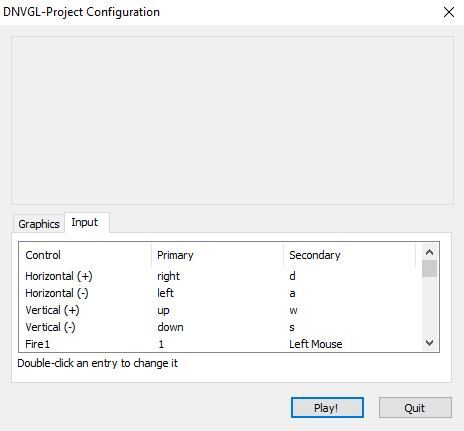
\includegraphics[width=\linewidth]{pictures/unity_build_startup.png}
\caption[The Unity Input Manager enable startup configuration]{The Unity Input Manager enables the user to specify which input keys to use for certain actions
when starting up the application}
\end{figure}


\subsection{The Raycast Controller}

\subsection{The Annotation Form Controller}
